\documentclass[letterpaper, 11pt]{article}

\usepackage[pdftex]{graphicx}
\usepackage{epstopdf}
\DeclareGraphicsRule{*}{mps}{*}{} 

\usepackage{amsmath, amsthm, amssymb}
\usepackage{listings}
\usepackage{float}
\usepackage{enumerate}
% \usepackage{mystyle}
\usepackage{hyperref}
\usepackage{tikz}
\usepackage{fancyheadings}
\usepackage{tensor}
\usepackage{mathrsfs}
\usetikzlibrary{positioning}
\usetikzlibrary{decorations.pathmorphing}
\usetikzlibrary{arrows}
\usetikzlibrary{decorations.markings}
%\usepackage{fullpage}
\usepackage[left=0.75in, top=1.25in, right=0.75in, bottom=1.25in]{geometry}
\newcommand{\lambdabar}{{\mkern0.75mu\mathchar '26\mkern -9.75mu\lambda}}

\numberwithin{equation}{section}
\numberwithin{figure}{section}

\begin{document}

\section{Magnetars}
\label{sec:magnetars}

\subsection{September 23}
\label{sec:sept-23}

Magnetars are pulsars with luminous X-ray emission and regular bursting behavior. The energy output is larger than the spin down power, which can only come from the magnetic field.

The spectrum of magnetars vary, but usually it consists of a soft component centered around $1\,\mathrm{keV}$, and a hard component in the MeV range. The soft component can usually be fit with a quasi-thermal spectrum with two blackbodies, but the hard X-ray emission in particular is non-thermal and has to be of magnetospheric origin.

The question is then, how is the energy released. If one simply work out the energistics, the total energy output of a magnetar is usually larger than or comparable to the total magnetic energy of the spin-down dipole field. So either the efficiency is very high, or the magnetic energy in the magnetosphere is replenished somehow. To be more precise, the dipole component of the magnetic field is not enough to provide the energy content of the bursts. Therefore people expect that there is much higher magnetic field inside the star, in configurations more convoluted than the dipole, for example a toroidally dominated configuration. There is some discussion about the maximum magnetic field you can have in a magnetar.

The surroundings of a magnetar is filled with plasma. Since the field is so high (even the spindown dipole field), it is easy to fill the magnetosphere. If the crust is deformed by some differential rotation, there will be twist of magnetic field lines building up in the magnetosphere. Assuming there is $B_{\phi}$ in the magnetosphere already, and to zeroth order $E_{\parallel}$ is zero, then the twist will live forever and there will simply be enough electric current to sustain $\nabla\times B$. In this limit there will be no dissipation and no radiation. To get energy dissipation and observable emission, one needs nonzero $\boldsymbol{E}\cdot \boldsymbol{j}$.

A better way to quantify the nonzero $\boldsymbol{E}$ is the voltage along the field lines, which is basically
\begin{equation}
    \label{eq:1}
    \Phi_e = \int \boldsymbol{E}\cdot d\boldsymbol{l}
\end{equation}
where the integral is along the magnetic field line. The question is how the twist of magnetic field will evolve in time and what kind of radiation will it emit.

The dynamics of the magnetosphere is govern by the following (simple) equations:
\begin{align}
  \frac{1}{c}\frac{\partial \boldsymbol{B}}{\partial t} &= -\nabla \times \boldsymbol{E} \\
  \frac{1}{c}\frac{\partial \psi}{\partial t} &= \frac{\partial \Phi_{\parallel}}{\partial t}
\end{align}
where $\psi$ is the twist. The twist is defined as the accumulative angle that the field line builds up:
\begin{equation}
    \label{eq:2}
    \psi = \int \frac{B_{\phi} d\boldsymbol{l}}{B r \sin\theta} = \int d\phi
\end{equation}
which is simply geometry. Now we let current flow along the magnetic field line, which must be maintained by a longitudinal voltage given by (\ref{eq:1}). If we consider to neighboring field lines and draw a closed loop by connecting the end points, then the rate of change of magnetic flux through the loop will be the circulation of $\boldsymbol{E}$ field along the loop. In the limit the two field lines are infinitely close, the voltage between end points is negligible, so
\begin{equation}
    \label{eq:3}
    \frac{d\delta\Phi}{dt} = \int E_{\parallel}dl_1 - \int E_{\parallel} dl_2
\end{equation}
The point is that, this time derivative of the differential flux $\delta\Phi$ only depends on $B_{\phi}$. One can see that by (some argument which we will talk about again next time). In the end what we can find is that
\begin{equation}
    \label{eq:4}
    \delta\Phi_{e} = \frac{\dot{\psi}(f)}{2\pi}\delta f
\end{equation}

\subsubsection{Discussion about the derivation}
\label{sec:disc-about-deriv}

There are two ways of deriving equation (\ref{eq:4}). Both start with considering a thin loop formed by points $P_1$, $P_2$ very close to each other on the star as footpoints of magnetic fieldlines, and the other footpoints $Q_1$ and $Q_2$ on the surface of the other hemisphere. The loop $\overline{P_1P_2Q_2Q_1}$ is what we want to integrate $E_{\parallel}$ along.

The first way is outlined in Andrei's review (which I failed to outline). The other way is what we discussed a lot about after the lecture. The problem is about the definition of the surface over which magnetic flux $\delta\Phi$ is computed. Since the magnetic field lines are moving with time, the flux surface bound by the field lines change, therefore the total derivative $d\delta\Phi/dt$ has two contributions, one from varying $B$ field, and the other from changing of the area itself.

If one considers a simple configuration of some $B$ field over an area, which is moved by $v\Delta t$, then we can find the expression for $d\Phi/dt$ by the following:
\begin{align}
  \Phi_t &= \int \boldsymbol{B}_t\cdot d\boldsymbol{S}_t \\
  \Phi_{t + \Delta t} &= \int \boldsymbol{B}_{t + \Delta t}\cdot d\boldsymbol{S}_{t + \Delta t}
\end{align}
Now in order to form a closed surface, we have $S_t$, $S_{t + \Delta t}$, and the loop formed by the boundaries of $S_t$ and $S_{t + \Delta t}$, with width $v\Delta t$. Integrating $\boldsymbol{B}_t$ over this surface will give zero flux. So we have
\begin{equation}
    \label{eq:5}
    0 = \int \boldsymbol{B}_t\cdot d\boldsymbol{S}_{t + \Delta t} - \int \boldsymbol{B}_t\cdot d\boldsymbol{S}_t + \oint \boldsymbol{B}_t\cdot (d\boldsymbol{l} \times \boldsymbol{v}\Delta t)
\end{equation}
where the last line integral is over the boundary of the area. Now we can see that the first two terms are almost $\Phi_{t + \Delta t} - \Phi_t$, only missing a $\Delta \boldsymbol{B}$ term, so we have
\begin{equation}
    \label{eq:6}
    \Phi_{t + \Delta t} - \Phi_t = \int \Delta \boldsymbol{B}\cdot d\boldsymbol{S} - \oint \boldsymbol{B}\cdot (d\boldsymbol{l}\times \boldsymbol{v}\Delta t)
\end{equation}
Note that we now omit the subscript $t$ on the right hand side, because everything is evaluated at time $t$. Dividing by $\Delta t$ and using Stoke's Theorem we get
\begin{equation}
    \label{eq:7}
    \frac{d\Phi}{dt} = \int \left[ \frac{\partial \boldsymbol{B}}{\partial t} - \nabla\times(\boldsymbol{v}\times \boldsymbol{B}) \right] d\boldsymbol{S}
\end{equation}

Now consider our problem of flux over the loop $\overline{P_1P_2Q_2Q_1}$. Since the boundaries $\overline{P_1Q_1}$ and $\overline{P_2Q_2}$ are along magnetic field lines, we can define the surface to be exactly along magnetic field lines. Therefore by construction $\Phi$ is identically zero. Since the field lines are moving, the time derivative of this $\Phi$ is given by equation (\ref{eq:7}). So by construction we have $d\Phi/dt = 0$:
\begin{equation}
    \begin{split}
        \frac{d\Phi}{dt} = 0 &= \int \left[ \frac{\partial \boldsymbol{B}}{\partial t} - \nabla\times(\boldsymbol{v}\times \boldsymbol{B}) \right]\cdot d\boldsymbol{S} \\
        &= -\int \nabla\times(\boldsymbol{E} + \boldsymbol{v}\times \boldsymbol{B})\cdot d\boldsymbol{S} \\
        &= -\oint (\boldsymbol{E} + \boldsymbol{v}\times \boldsymbol{B})\cdot d\boldsymbol{l}
    \end{split}
\end{equation}
In other words, the ``comoving electric field'' integrates to zero along the loop.

If one proceeds with the last line, we have
\begin{equation}
    \label{eq:8}
    \oint \boldsymbol{E}\cdot d\boldsymbol{l} = - \oint (\boldsymbol{v}\times \boldsymbol{B})\cdot d\boldsymbol{l}
\end{equation}
Consider the left hand side. If we make the assumption that the stellar surface is a good conductor, inside which $\boldsymbol{E}$ vanishes, then the integral of $\boldsymbol{E}$ along the loop becomes
\begin{equation}
    \label{eq:9}
    \oint \boldsymbol{E}\cdot d\boldsymbol{l} = \int_{P_2Q_2}\boldsymbol{E}\cdot d\boldsymbol{l} - \int_{P_1Q_1}\boldsymbol{E}\cdot d\boldsymbol{l} = \int E_{\parallel} dl_2 - \int E_{\parallel} dl_2 = \delta \Phi_{e}
\end{equation}
which is the difference of the voltage drops along the adjacent field lines. The right hand side of equation (\ref{eq:8}) can be written as $-\oint (\boldsymbol{B}\times d\boldsymbol{l})\cdot \boldsymbol{v}$, which obviously vanishes along the field lines, and is nonzero only on the small segments on the stellar surface. If we further assume that the points $P_1$ and $P_2$ are fixed on the stellar surface, with only their other footpoints $Q_1$ and $Q_2$ moving due to evolving magnetic field, and the evolution of the footpoints is evolution of the twist $\psi$, then the right hand side of equation (\ref{eq:8}) can be written as
\begin{equation}
    \label{eq:10}
    - \oint (\boldsymbol{v}\times \boldsymbol{B})\cdot d\boldsymbol{l} = - \int_{Q_1Q_2}(\boldsymbol{B}\times d\boldsymbol{l})\cdot \boldsymbol{v} = \int_{Q_2Q_1}(r_{\perp}\dot{\psi}B_p)dl
\end{equation}
Finally we identify the poloidal flux $\delta f = \int 2\pi r_{\perp}B_pdl$, so that we have
\begin{equation}
    \label{eq:11}
    \delta \Phi_e = \frac{\dot{\psi}\delta f}{2\pi}
\end{equation}
which is exactly the result (\ref{eq:4}) Andrei obtained.

A good extension of this formalism is that, if we assume finite conductivity inside the star, then it is very easy to modify the end result (\ref{eq:11}). We just need to add a resistive term to the integral of $\boldsymbol{E}$, which modifies $\delta \Phi_e$.

\subsection{September 28}
\label{sec:sept-28}

To extend the discussion about the untwist problem. Apart from the discussion above, there is the original Andrei's formalism. The way is to consider the magnetic flux only across the meridional plane. The toroidal flux function across the same magnetic loop $\overline{P_1P_2Q_2Q_1}$ is
\begin{equation}
    \label{eq:12}
    F = \int B_{\phi}dl ds = \int \frac{B_{\phi}dl\delta f}{2\pi r_{\perp}B_{p}} = \frac{\psi \delta f}{2\pi}
\end{equation}
where $dl$ is along the field line and $ds$ is across the field line. This result is a geometrical identity
\begin{equation}
    \label{eq:13}
    \psi = \frac{1}{2\pi}\frac{\partial F}{\partial f}
\end{equation}
To get the original result we take the derivative of this equation with respect to time
\begin{equation}
    \label{eq:14}
    \dot{\psi} = \frac{1}{2\pi}\partial_f\partial_tF = \frac{1}{2\pi}\partial_f\frac{dF}{dt} 
\end{equation}
The last equality is because $F$ is a function of $f$ and $t$, but the time evolution of $F$ is due to the breathing of the field lines, so the time derivative of $F$ is simply the total time derivative. Now we have
\begin{equation}
    \label{eq:15}
    \frac{dF}{dt} = \oint \boldsymbol{E}'_p\cdot d\boldsymbol{l}_p = \oint \boldsymbol{E}\cdot d\boldsymbol{l} = \delta\Phi_e
\end{equation}
where $E'$ means the electric field in the frame comoving with the magnetic field lines.

A crucial argument to this method is that, to justify the last equation that our integration of $E_{\parallel}$ is correct, we need $E'_{\phi} = 0$. This is true because if we decompose the magnetic field into poloidal and toroidal components
\begin{equation}
    \label{eq:16}
    \boldsymbol{B} = \frac{\nabla f\times \boldsymbol{e}_{\phi}}{2\pi} + B_{\phi}\boldsymbol{e}_{\phi}
\end{equation}
by the ``frozen-in condition'' we have
\begin{equation}
    \label{eq:17}
    \frac{\partial \boldsymbol{B}}{\partial t} = \nabla\times(\boldsymbol{v}\times \boldsymbol{B})
\end{equation}
therefore for the $\boldsymbol{v}_p$ of the field line in the poloidal component we can find $E'_{\phi}$ such that
\begin{equation}
    \label{eq:18}
    \partial_t\boldsymbol{E}'_{\phi} = \partial_t\boldsymbol{E} + \boldsymbol{v}_p\times \boldsymbol{B}_p = 0
\end{equation}

\subsubsection{Discharge}
\label{sec:discharge}

The next logical step is to figure out what controls the voltage drop. That is connected to the discharge mechanism. The equation (\ref{eq:11}) tells us that (filling the missing $c$ back)
\begin{equation}
    \label{eq:19}
    \dot{\psi} = 2\pi c\frac{\partial \Phi_e}{\partial f}
\end{equation}
Therefore the larger the voltage, the faster the untwisting. (Is this really true? It's only the derivative of voltage entering the equation.)

Consider axisymmetric configuration, the total poloidal current $I$ over a field line bundle is the circulation of $B_{\phi}$. The first question is that whether this current is possible to be sustained by particles extracted from the surface. The picture by Thompson and Duncan is that the particles supplied from the surface is sufficient to carry the current. To work out this problem one needs to consider gravity.

The minimum number density of particles to conduct a certain current is given by $n_{min} = j/ec$. The voltage produced by missing this amount of charge is given by
\begin{equation}
    \label{eq:20}
    \Phi_{e} \sim 4\pi e n_{min}R^2 = 4\pi R^2\frac{j}{c}
\end{equation}
This is loosely applying the Maxwell equation
\begin{equation}
    \label{eq:21}
    \nabla\times \boldsymbol{B} = \frac{4\pi}{c}\boldsymbol{j} + \frac{1}{c}\frac{\partial \boldsymbol{E}}{\partial t}
\end{equation}
by assuming that $\boldsymbol{B}$ is extremely large, and that $\nabla\times \boldsymbol{B}$ is given. The plasma has to figure out a way to sustain this curl of $\boldsymbol{B}$, which is the current the field demands, and we call it $\boldsymbol{j}_{B} = n_{min}ec$. If we have vacuum instead of this amount of charge, and we want to find the characteristic electric field associated to this missing amount of charge is given by equation (\ref{eq:20}).

Another way (better way) to look at the equation (\ref{eq:21}) is
\begin{equation}
    \label{eq:22}
    \frac{\partial E_{\parallel}}{\partial t} = 4\pi(j_B - j)
\end{equation}
so it says if we don't have the desired $j$, the electric field grows. Let's look at the time scale associated with the missing $j$. Over a characteristic time $\tau$, assuming initially we have some plasma but with $v = 0$, we have
\begin{align}
  \frac{E_{\parallel}}{\tau} &\sim 4\pi (j_B - j) \\
  \tau e E_{\parallel} &\sim mv \sim mj/ne
\end{align}
putting these equations together we have
\begin{equation}
    \label{eq:23}
    \tau^2 \sim \frac{m j}{4\pi e^2n(j_B - j)} = \frac{1}{\omega_p^2}\frac{j}{j_B - j}
\end{equation}
So the time scale is comparable to the plasma time scale, which is very short. The morale is that the plasma responds to missing current very quickly, so electric field develops very quickly in response to any mismatch of $j_{B}$ and $j$. If we estimate the plasma frequency
\begin{equation}
    \label{eq:24}
    \omega_p^2 = \frac{4\pi e^2n}{m_e} \sim \frac{4\pi e j}{m_ec} \sim \frac{eB}{m_eR}, \quad \omega_{p} \sim 10^{13}B_{15}^{1/2}\,\mathrm{rad/s}
\end{equation}
which is much smaller compared to the light crossing time of the system.

If we look for a steady state where some $E_{\parallel}$ overcomes gravity to pull enough charges from the star to conduct the current, we will find that it is actually impossible. The continuity equations for the charges, together with divergence of $B$ being zero, we have $\nabla\cdot \boldsymbol{j}_{\pm} = \nabla\cdot \boldsymbol{B} = 0$ because the $\partial_t(n_{\pm}e)$ term in the continuity equation is zero. Because $j$ is parallel to $B$, let $\boldsymbol{j} = \alpha \boldsymbol{B}$, we have
\begin{equation}
    \label{eq:25}
    \nabla\cdot \boldsymbol{j}_{\pm} = (\boldsymbol{B}\cdot\nabla)\alpha = \frac{\partial}{\partial l}\frac{j_{\pm}}{B}
\end{equation}
so $\alpha$ is constant along the field line. This means that $n_{\pm}v_{\pm}/B$ is constant along field lines, so if $n_+ = n_-$ in the atmosphere, we have
\begin{equation}
    \label{eq:26}
    \frac{j_+}{j_-} = -\frac{v_+}{v_-} = \mathrm{const}
\end{equation}
The argument is that, if there is some $E_{\parallel}$ that pulls out the particles from the surface self-consistently, then you can't have $v_+/v_-$ to be constant everywhere. For example $v_+$ is zero at one footpoint, with $v_-$ nonzero, but the opposite is true at the other footpoint.

\subsection{September 30}
\label{sec:sept-30}

\subsubsection{About annihilation}
\label{sec:annihilation}

At the end of last meeting there was a question about the possibility of pair annihilation in the current bundle. Let's estimate the particle density in more detail here. Consider a twisted dipole magnetosphere. On a given dipole field line the $r$ and $\theta$ are related by $r = R_\mathrm{max}\sin^2\theta$. Given a twist $\psi$, the current flowing will be (assuming $\psi$ is relatively small, $\psi < 1$, so that the global field is still approximately dipole)
\begin{equation}
    \label{eq:27}
    j = \frac{c\psi B}{4\pi R_\mathrm{max}},\quad n_e = \frac{\psi B}{4\pi\beta e R_\mathrm{max}}
\end{equation}
The flux function for dipole field is simply $f = f_\mathrm{max}\sin^2\theta$. This is relatively simple to compute since one can just integrate the $B$ field flux over the surface up to angle $\theta$.

If we write $u = f/f_\mathrm{max} = \sin^2\theta$, which is essentially rescaled $f$, then we can write
\begin{equation}
    \label{eq:28}
    j = \frac{R B}{2\pi \mu} \frac{\partial I}{\partial u},\quad I = \frac{\psi c\mu u^2}{4R^2}
\end{equation}

From equation \eqref{eq:27} we can get a numerical value of then particle density:
\begin{equation}
    \label{eq:29}
    n_e = \psi \times 10^{16}\frac{B}{B_Q}\left( \frac{R_6}{R_\mathrm{max}} \right) \mathrm{cm}^{-3}
\end{equation}
where $B_Q$ is the critical field $B_Q = 4.4\times 10^{13}\,\mathrm{G}$.

Now we consider pair annihilation. An electron-positron pair can collide and turn into a pair of photons. The cross section will be inversely proportional to their relative velocity, and the rate of annihilation will be proportional to the cross section times $v$, so the rate of annihilation in weak field ($B/B_Q\ll 1$) and vacuum will be
\begin{equation}
    \label{eq:30}
    \mathcal{R}_{0}^{(2)} = \sigma_\mathrm{ann}v \sim 1.5\times 10^{-14} \mathrm{cm^3/s} \sim 0.1\sigma_Tc
\end{equation}

However, when $B$ is not far smaller than $B_Q$, the formula needs to be changed. If $B \gtrsim 2B_Q$, we have
\begin{equation}
    \label{eq:31}
    \mathcal{R}^{(2)} = \frac{1.74 \mathcal{R}_0}{b^3}\exp \left( -\frac{2}{b} \right)
\end{equation}
where $b = B/B_Q$. So in strong field this rate is suppressed by a coefficient of $b^{-3}$. This was first done by \href{http://adsabs.harvard.edu/abs/1979PhRvL..42...79W}{Wunner} in 1979. There are a few more papers, e.g. \href{http://adsabs.harvard.edu/abs/1987Ap%26SS.138....1K}{(Kaminker et. al. 1987)}.

In strong field there is an additional process, which is 1-photon annihilation, which is one pair annihilating into a single photon. Normally this is not allowed due to conservation of energy and momentum, but the magnetic field can take the extra momentum. Wunner reported the result for the ratio between 1-photon and 2-photon annihilation:
\begin{equation}
    \label{eq:32}
    \frac{\mathcal{R}^{(1)}}{\mathcal{R}^{(2)}} = 496b^{2}
\end{equation}
So 1-photon annihilation is much more efficient than the 2-photon annihilation in strong field. The overall rate is dominated by 1-photon annihilation, and it scales with $b^{-1}$ when $B/B_Q>1$.

The most important region for pair annihilation is when $b\gtrsim 1$ because when $B$ is too large the rate is suppressed. The change of $n_\pm$ due to annihilation can be estimated as:
\begin{equation}
    \label{eq:33}
    \frac{\Delta n_\pm}{n_\pm} \sim \frac{r}{c}\frac{\dot{n}_\mathrm{ann}}{n_\pm} \sim \frac{r}{c}\mathcal{R}n_e \sim \frac{0.1\psi}{R_7/R_{max}}
\end{equation}
where $n_e$ is given by equation \eqref{eq:29}.

\subsubsection{Double layer}
\label{sec:double-layer}

Consider a 1D box with conductor at both ends. If one pushes some current $j$ at the ends of the box, and we have plenty of plasma in the box, then electric field will be induced and pushes the plasma to conduct the current $j$. However for a neutron star, originally we don't have much plasma around the star, except in a very thin atmosphere near the surface. The scale height of the atmosphere should be
\begin{equation}
    \label{eq:34}
    h \sim \frac{kT}{gm_p} \sim 1\,\mathrm{cm}
\end{equation}
where $g$ is the surface gravity of the neutron star $g \sim GM/R^2 \sim 10^{14}cm/s^2$. This gravity is very weak. The electric field that one needs to offset this gravity is orders of magnitude less than $B$. As discussed last time, there is no self-consistent solution for a steady electric field to help conduct the current required by the boundary condition. The result is that the system will relax to what is called a ``double layer''.

Let's assume the current is conducted by negative and positive charge $j = j_{-} + j_{+}$, and that $j_+ = j_-$. So we have
\begin{equation}
    \label{eq:35}
    n_{\pm} = \frac{j_{\pm}}{ev_{\pm}} = \frac{j}{2ev_{\pm}}
\end{equation}
Near the anode $v_-\approx c$ while $v_+\sim 0$ which means $n_+\gg n_-$, so the charge density is $\rho \sim en_{+}$. High density translates to high electric field due to Gauss's law $4\pi\rho = \partial_zE$, and the charges will quickly accelerate and charge density quickly decreases. Near the surface we have $E_z \sim \rho z \sim jz/v$. The work done by the electric field will be
\begin{equation}
    \label{eq:36}
    zEe \sim \frac{mv^2}{2}, \quad v(z) \sim \sqrt[3]{\frac{ejz^2}{m}}
\end{equation}
So velocity is proportional to $z^{2/3}$, and $\rho \sim e n_+ \sim z^{-2/3}$. This holds up to the point where $v \sim c$. At this point $v$ stops growing, and $n_+$ should match $n_-$ so that $\rho \sim 0$. For relativistic case we can find that
\begin{equation}
    \label{eq:37}
    \gamma \sim \frac{ejz^2}{mc^{3}}
\end{equation}
The thickness of the acceleration layer, which is the $z$ position where $v$ becomes $c$ can be found by
\begin{equation}
    \label{eq:38}
    z^2\sim \frac{mc^2ce}{e^2j} \sim c^2\frac{m}{n_0e^2} \sim c^2/\omega_{p}^2
\end{equation}
where $n_0$ is a characteristic number density in the layer. The solution is that opposite charges are concentrated at the two ends of the box, and provide the acceleration electric field in between. The charges are highly concentrated in a small scale comparable to the plasma skin depth. There is huge electric field in between, which can be estimated as
\begin{equation}
    \label{eq:39}
    E \sim 4\pi\rho z \sim \frac{4\pi j}{\omega_p}
\end{equation}
we can find the potential corresponding to this electric field
\begin{equation}
    \label{eq:40}
    \frac{e\Phi_e}{mc^2} = \frac{4\pi j eR}{\omega_pmc^2} = \frac{\omega_p}{c}R = \frac{R}{\lambda_p}
\end{equation}
This voltage is huge. We estimated $\omega_p\sim 10^{13}\,\mathrm{rad/s}$, so that this voltage is around $10^9$. This is the double layer solution found by \href{http://adsabs.harvard.edu/abs/1982Ap%26SS..87...21C}{Carlqvist} in 1982.

Note that if we turn off gravity then with any finite temperature we don't have this structure. At any given temperature then scale height of the atmosphere is infinite, so the particles can freely stream out from the star to conduct the current. Even with gravity, if it is weak enough, in other words if the density at the top of the scale height is sufficient to conduct the current
\begin{equation}
    \label{eq:41}
    \frac{n_\mathrm{atm}}{n_0} = \frac{n_\mathrm{atm}^0\exp(-z/h)}{j/ec} > 1
\end{equation}
then it is possible to conduct the current without forming the double layer.

\subsection{October 5}
\label{sec:oct-5}

We established that if the current can't be conducted, a double layer will be formed with large electric field. The electric field will accelerate particles which induces pair creation.

\subsubsection{Resonant scattering}
\label{sec:res-scatter}

In magnetars the dominant pair creation process is resonant scattering, as opposed to curvature radiation in standard pulsars. In the former case an electron moving at Lorentz factor $\gamma$ scatters a seed photon at energy $\hbar\omega$ to energy $\gamma^2\hbar\omega$, which then convert to an electron-positron pair. In the later the particles move along curved field lines and emit curvature radiation at energy $\hbar c\gamma^3/R_c$. The reason that curvature radiation is subdominant (or straight negligible) in magnetars is that $\gamma$ doesn't reach high enough values. For curvature radiation to be high enough energy to produce pairs, $\gamma$ needs to be on the order of $\gtrsim 10^6$, whereas for resonant scattering the Lorentz factor required is much lower, at the order of $\sim 10^3$.

The physics of resonant scattering is simply the interaction of an oscillating particle in magnetic field interacting with radiation. Consider an oscillator under external harmonic force, the equation of motion is
\begin{equation}
    \label{eq:42}
    \ddot{x} + \omega_0^2x = \frac{eE}{m}
\end{equation}
using Fourier transform we can find
\begin{equation}
    \label{eq:43}
    x = \frac{eE}{m(\omega_0^2 - \omega^2)}, \quad \ddot{x} = \frac{eE\omega^2}{m(\omega_0^2 - \omega^2)}
\end{equation}
In this kind of classic scattering cross section, we have near resonance
\begin{equation}
    \label{eq:44}
    \frac{d\sigma}{d\Omega'} = r_e^2\frac{\omega^2}{(\omega - \omega_B)^2} \left| \boldsymbol{e}^{*}\cdot \boldsymbol{e}_- \right|^2 \left| \boldsymbol{e}'^{*}\cdot \boldsymbol{e}_- \right|^2
\end{equation}
where $r_e$ is the classical electron radius and $\omega_B = eB/m_ec$. The factor $r_e^2$ enters because this is to some extent like a Thomson scattering with incoming and outgoing photons.
$\boldsymbol{e}$ and $\boldsymbol{e}'$ are the polarization vectors of the incoming and outgoing waves, and $\boldsymbol{e}_-$ is the vector corresponding to the electron orbit direction.

This equation \eqref{eq:44} is singular when $\omega = \omega_B$ which is exactly the case we are interested in. The way to view what is happening at resonance is to look at quantum mechanically. We can think of the scattering as a two-step process: the electron first absorbs a photon, and then spontaneously emits a photon. The classical cross section needs to be modified by a factor of $\Gamma$ which is related to the lifetime of the electron in the excited state:
\begin{equation}
    \label{eq:46}
    \frac{\omega^2}{(\omega - \omega_B)^2} \longrightarrow \frac{\omega^2}{(\omega - \omega_B)^2 + (\Gamma/2)^2}
\end{equation}
If we define $B_Q = m_e^2c^3/\hbar e$ as the critical field, the energy difference between the lowest and second lowest Landau levels is $\hbar\omega_B$ when $B\ll B_Q$, and it becomes
\begin{equation}
    \label{eq:45}
    \left[ \left( 1 + 2\frac{B}{B_Q} \right)^{1/2} - 1  \right] m_ec^2
\end{equation}
The correction $\Gamma$ will be given by
\begin{equation}
    \label{eq:47}
    \frac{\Gamma}{\omega_B} = \frac{4}{3}\alpha\frac{B}{B_Q}
\end{equation}
which was found in \href{http://adsabs.harvard.edu/abs/1982A%26A...115...90H}{(Herold et. al. 1982)}. When $\hbar\omega_B$ becomes comparable to $m_ec^2$ the formula \eqref{eq:46} needs to be changed, which was considered in \href{http://adsabs.harvard.edu/abs/1979PhRvD..19.2868H}{(Herold 1979)}.

If we plug equation \eqref{eq:47} into equation \eqref{eq:46} and take the limit $\Gamma \to 0$ (or equivalently $\Gamma\ll \omega_B$), we get
\begin{equation}
    \label{eq:48}
    \frac{1}{(\omega - \omega_B)^2 + (\Gamma/2)^2}\longrightarrow\frac{2\pi}{\Gamma}\delta(\omega - \omega_B)
\end{equation}
so obviously the cross section peaks at $\omega = \omega_B$.

If we define $\mu = \cos\theta$ and $\mu' = \cos\theta'$ where $\theta$ and $\theta'$ are angles of incoming and outgoing photons with respect to the magnetic field, then the cross section should be written as (if the electron is at rest)
\begin{equation}
    \label{eq:49}
    \frac{d\sigma}{d\mu'} = 3\pi^2r_ec\delta(\omega - \omega_B)\left| \boldsymbol{e}^{*}\cdot \boldsymbol{e}_\pm \right|^2 \left| \boldsymbol{e}'^{*}\cdot \boldsymbol{e}_\pm \right|^2
\end{equation}

We can define two linear polarizations for a photon in the magnetic field, which have slightly different propagation speeds. Given $\boldsymbol{B}$ and $\boldsymbol{k}$ vectors, we can have $\boldsymbol{E}$ vector in the plane of $\boldsymbol{B}$-$\boldsymbol{k}$, which we call ``O'' mode, or parallel mode, and $\boldsymbol{E}$ perpendicular to the plane of $\boldsymbol{B}$-$\boldsymbol{k}$, which we call ``E'' mode, or perpendicular mode. The refraction indices of these two modes are different:
\begin{align}
    \label{eq:50}
  N_{\perp} &= 1 + \frac{2\alpha}{45\pi} \left( \frac{B}{B_Q} \right)^2\sin^2\theta \\
  N_{\parallel} &= 1 + \frac{7\alpha}{90\pi} \left( \frac{B}{B_Q} \right)^2\sin^2\theta
\end{align}
If we integrate equation \eqref{eq:49} over $\theta'$ and sum over outgoing photon polarizations we can find the total cross section
\begin{equation}
    \label{eq:51}
    \sigma_\mathrm{tot} = \sum_{\boldsymbol{e}'}\int_{-1}^1\frac{d\sigma}{d\mu'}d\mu' = 2\pi^2 r_e c\xi \delta(\omega - \omega_B)
\end{equation}
where $\xi$ is 1 for perpendicular mode and $\xi$ is equal to $\mu^2$ for parallel mode. This is due to pure geometry and come from the $\boldsymbol{e}\cdot \boldsymbol{e}_{\pm}$ factor. This final result applies not only for $B\ll B_Q$ but also for $B$ comparable to or larger than $B_Q$, if the incoming photon is along the $B$ field. If the photon is at some angle with respect to the field then the cross section needs to be corrected. If one wants we can convolute this result with some frequency distribution, and we can find a rate for resonant scattering
\begin{equation}
    \label{eq:52}
    \dot{n}_\mathrm{res} \sim n_e n_\mathrm{ph}\sigma^\mathrm{res}_\mathrm{eff}c
\end{equation}
where
\begin{equation}
    \label{eq:53}
    \sigma^\mathrm{res}_\mathrm{eff} \approx \frac{2\pi^2r_ec}{\omega_B}
\end{equation}
compare this with Thomson cross section
\begin{equation}
    \label{eq:54}
    \sigma_T \approx \frac{8\pi}{3}r_e^{2}
\end{equation}
so for $B$ larger than critical field this resonant cross section is larger than the normal Thomson cross section.

\subsection{October 7}
\label{sec:oct-7}

If one takes equation \eqref{eq:51} and rewrite equation \eqref{eq:49} we can write
\begin{equation}
    \label{eq:55}
    \frac{d\sigma}{d\mu'} = \sigma_\mathrm{tot} \frac{3}{8}\xi'
\end{equation}
and the parallel polarization takes 3/4 of the outgoing power.

Since the result \eqref{eq:51} does not depend on the smallness of $B/B_Q$, it is valid even for $b> 1$, which is puzzling because in high magnetic field the Landau level gets corrected as given by equation \eqref{eq:45}. Nevertheless in the formula the resonance condition is still $\omega = \omega_B$. This is because recoil in scattering. Consider a photon coming along the $B$ field scatter off an electron. We define $\epsilon_B = \sqrt{1 + 2b}$, which is the dimensionless Landau energy. Let $\epsilon_0 = E_{\gamma}/m_ec^2$ be the initial photon energy in the electron rest frame. The first part of the scattering process is absorption of the photon, giving total energy $\epsilon_0 + 1$ in the initial rest frame of the electron. After absorption, the electron is now moving with some Lorentz factor $\gamma$, and we have conservation of both energy and momentum:
\begin{equation}
    \label{eq:56}
    \epsilon_0 + 1 = \gamma\epsilon_B,\quad \epsilon_0 = \gamma\beta\epsilon_B
\end{equation}
where the equations are written in the initial rest frame of the electron. One can solve this set of equations for $\epsilon_0$ and $\gamma$ since they tell us the resonance condition, and the recoil
energy of the electron:
\begin{equation}
    \label{eq:58}
    \beta = \frac{b}{1 + b},\quad \gamma = \frac{1 + b}{\epsilon_B}, \quad \epsilon_0 = b
\end{equation}
Note again that this is assuming the photon comes in along the magnetic field. In this case the resonance condition is simply $\omega = \omega_B$.

\subsubsection{Discharge mechanism}
\label{sec:discharge-mech}

We started this discussion of resonance scattering because we wanted to see how the particles in the double layer configuration produce pairs. In that physical situation, the accelerated electrons in moving along the $B$ field will upscatter photons from the stellar surface and undergo the resonance scattering process to produce higher energy photons which are capable of producing electron-positron pairs.

Given what we've calculated so far, we want to compute the free path of an electron at Lorentz factor $\gamma$. The scattering rate per second is an integration:
\begin{equation}
    \label{eq:59}
    \dot{N}_\mathrm{sc} = \int d\Omega \int d\omega \frac{I(\hbar\omega)}{\hbar\omega}\sigma_\mathrm{tot}
\end{equation}
where $I$ is the intensity of photons, namely the energy flux of photons per area at a given solid angle, so $I/\hbar\omega$ is the number flux across unit area. Note that our $\sigma_\mathrm{tot}$ was derived in the rest frame of the electron, whereas we need the cross section in the lab frame. We need to transform this cross section by a factor of $(1 - \beta\mu)$. The cross section is suppressed when the photon is traveling at the same direction as the electron, when $\mu \sim 1$. Another correction is for $\omega$ in the rest frame of the electron, which is related to the lab frame photon frequency by
\begin{equation}
    \label{eq:57}
    \tilde{\omega} = \gamma(1 - \beta\mu)\omega
\end{equation}
where $\tilde{\omega}$ is the Lorentz transformed frequency in the electron rest frame. In the rest frame of the electron, due to relativistic effect, the photon is either coming from the front or the back of the electron along the field line, so $\mu$ will be either 1 or $-1$, and $\xi \sim 1$. So we can carry out the integral:
\begin{equation}
    \label{eq:60}
    \begin{split}
        \dot{N}_\mathrm{sc} &= \int d\Omega \int d\omega 2\pi^2 r_ec\frac{\delta(\omega - \tilde{\omega}_B)}{|d\tilde{\omega}/d\omega|}(1 - \beta\mu)\frac{I}{\hbar\omega} \\
        &= \int d\Omega \int d\omega 2\pi^2 r_ec \delta \left( \omega - \frac{\omega_B}{\gamma(1 - \beta\mu)} \right)\frac{I}{\gamma\hbar\omega} \\
        &= \int d\Omega \frac{2\pi^2 r_ec}{\gamma}\frac{I(\omega_\mathrm{res})}{\hbar\omega_\mathrm{res}}
    \end{split}
\end{equation}
where $\omega_\mathrm{res}$ is the boosted $\omega_B$:
\begin{equation}
    \label{eq:61}
    \omega_\mathrm{res} = \frac{\omega_B}{\gamma(1 - \beta\mu)}
\end{equation}
Sufficiently far away from the star, the star subtends only a relatively small solid angle, and we can finish the integral and get
\begin{equation}
    \label{eq:62}
    \dot{N}_\mathrm{sc} = \frac{2\pi^3r_ec}{x^2\gamma}\frac{I(\omega_\mathrm{res})}{\omega_\mathrm{res}}
\end{equation}
where $x = r/R_{*}$. The radiation from the star is predominantly in perpendicular mode, and assuming Planck spectrum we have
\begin{equation}
    \label{eq:63}
    I_{\perp} = \frac{\hbar\omega^3}{8\pi^3c^2 \left[ \exp \left( \hbar\omega/kT - 1 \right) \right]}
\end{equation}
so we can write the rate as
\begin{equation}
    \label{eq:64}
    \dot{N}_\mathrm{sc} = \frac{\alpha\Theta c}{4x^2\gamma \lambdabar}\frac{g(y)}{y}
\end{equation}
where $\Theta = kT/m_ec^2$, $g(y) = y^3/(e^y - 1)$, and $y = h\omega_\mathrm{res}/kT$, and $\lambdabar$ is the electron Compton wavelength $\lambdabar = \hbar/m_ec$. If we multiply this with the characteristic time which is $t \sim r/c$, then the total number of scattering is huge because of a factor of $R/\lambdabar$ which gives the multiplicity. For typical magnetar parameters this will give about $10^5$.

Last question we want to ask is how the momentum changes due to scattering. The momentum change of an electron $\Delta p$ due to scattering in the lab frame is related to the momentum change in the rest frame of the particle $\Delta \tilde{p}$ by $\Delta p = \gamma \Delta \tilde{p}$. In the rest frame of the electron the incoming photon has a well-defined momentum $\hbar\omega_B$ but on average the outgoing photon has zero momentum because it can go in any direction. So on average the momentum that is given to the electron in the rest frame by the photon is
\begin{equation}
    \label{eq:65}
    \Delta \tilde{p} = \frac{\hbar\omega_B}{c}\tilde{\mu}
\end{equation}
where $\tilde{\mu}$ is the transformed $\mu$ into the electron rest frame
\begin{equation}
    \label{eq:68}
    \tilde{\mu} = \frac{\mu - \beta}{1 - \beta\mu}
\end{equation}
where $\mu$ is the angle of photon with respect to the magnetic field line. The momentum change to the electron in the lab frame is then $\Delta p = \gamma \Delta \tilde{p}$. If we multiply this to the scattering rate then we can get a force
\begin{equation}
    \label{eq:66}
    \mathcal{F} = \dot{N}_\mathrm{sc}\Delta p \propto \gamma(\mu - \beta)
\end{equation}
where $\mu$ is cosine of the angle between the photon coming from the star and the direction of the magnetic field. So the relationship of $\mu$ and $\beta$ of the electron determines the direction of the force. For most of the relativistic electrons this creates a huge drag force on the particles. The drag coefficient
\begin{equation}
    \label{eq:67}
    \mathcal{D} = \frac{r}{c}\frac{1}{p}\frac{dp}{dt} \gg 1
\end{equation}

\subsection{October 12}
\label{sec:oct-12}

Last time we derived the resonance scattering rate $\dot{N}_\mathrm{sc}$ \eqref{eq:63}. This rate is regulated by the intensity of thermal radiation at the particle position at the resonance frequency. Plugging in the Plank distribution we get equation \eqref{eq:64}, which peaks at the Wien peak where $g(y)/y \sim 1$ at $y \sim 2$. $\Theta \sim 10^{-3}$ is typical for magnetars where the stellar temperature is around $\mathrm{keV}$.

One can estimate the multiplicity of scattered photons by multiplying the rate by a characteristic time, which is the time it takes for a seed particle to cross a characteristic distance where $B$ is not changed by much. We can find (taking $\Delta r\sim r/3$):
\begin{equation}
    \label{eq:69}
    \mathcal{M}_{\gamma}(r)\sim \frac{\Delta r}{c}\dot{N}_\mathrm{sc} \sim \frac{\alpha\Theta^2R_{*}}{12 x \gamma}\frac{R_{*}}{\lambdabar}\frac{g(y)}{y} \sim \frac{10^7}{x\gamma} \gg 1
\end{equation}
For typical parameters this multiplicity is very high.

We can also find the drag force due to resonance scattering felt by the electron:
\begin{equation}
    \label{eq:70}
    \mathcal{F} = \dot{N}_\mathrm{sc}\Delta p = \dot{N}_\mathrm{sc}\gamma \Delta \tilde{p}
\end{equation}
where $\Delta \tilde{p}$ is the change of momentum in the rest frame of the electron. If the incoming photon angle in the rest frame is $\tilde{\mu}$ then $\Delta \tilde{p} = \tilde{\mu}\hbar\tilde{\omega}/c$. Plugging this in we get
\begin{equation}
    \label{eq:71}
    \mathcal{F} = \frac{\alpha^2}{4x^2}\frac{m_ec^2}{r_e}\Theta^3 \gamma g(y)(\beta_{*} - \beta)
\end{equation}
where $\beta_{*} = \mu$ is the incoming photon angle. This formula is applicable when $b \ll 1$. We will talk about the correction to this formula at critical field when pair creation is important.

We can find the drag coefficient which is the ratio of the drag timescale and the time scale of motion, which measures the importance of drag:
\begin{equation}
    \label{eq:72}
    \mathcal{D} = \frac{r}{c}\frac{1}{p}\frac{dp}{dt}
\end{equation}
If one finds that $\mathcal{D} \gg 1$, then the drag dominates, and eventually the radiation force will push the particle to the equilibrium velocity $\beta = \beta_{*}$, where $\mathcal{F} = 0$. Around this equilibrium, assuming $\left| \beta - \beta_{*} \right| \ll \beta_{*}$ we can expand and find
\begin{equation}
    \label{eq:73}
    \mathcal{D} = \mathcal{D}_{*} \left( 1 - \frac{p}{p_{*}} \right) = \frac{\alpha^2 R}{4 r_e}\frac{\Theta^3g(y_{*})}{x\gamma_{*}^2} \left( 1 - \frac{p}{p_{*}} \right)
\end{equation}
The coefficient $\mathcal{D}_{*}$ can be find to be
\begin{equation}
    \label{eq:74}
    \mathcal{D}_{*} = \frac{4\times 10^4}{x}\frac{g(y_{*})}{\gamma_{*}^2} \left( \frac{kT}{0.5\,\mathrm{keV}} \right)^3
\end{equation}

One other quantity we are interested in is the optical depth of radiation in the plasma-filled magnetosphere. If we assume that in the magnetosphere where plasma is moving with $\beta = \beta_{*}$ everywhere, we can find that
\begin{equation}
    \label{eq:75}
    \frac{d\tau}{ds} = \sigma_\mathrm{tot} n = n 2\pi^2r_ec\xi(1 - \beta\mu)\delta(\tilde{\omega} - \omega_B)
\end{equation}
where $s$ is the path length along the photon trajectory. To carry out the integral we can convert $ds$ to $d(\tilde{\omega} - \omega_B)$
\begin{equation}
    \label{eq:76}
    \delta(\tilde{\omega} - \omega_B)ds \longrightarrow \frac{\delta(\tilde{\omega} - \omega_B)d(\tilde{\omega} - \omega_B)}{\left| \frac{d(\tilde{\omega} - \omega_B}{ds} \right|}
\end{equation}
We want to argue that $d\tilde{\omega}/ds = 0$ for dipole field. Note that $\tilde{\omega} = \omega\gamma(1 - \beta\mu)$. When $\beta = \beta_{*}$ we can see that $\tilde{\omega} = \omega / \gamma_{*}$ which is only a function of $\theta$. However photons move in the radial direction along which $\theta$ is constant, we do see that $d\tilde{\omega}/ds = 0$. Therefore we can find
\begin{equation}
    \label{eq:77}
    \tau = \frac{2\pi^2r_ecn\xi(1 - \beta\mu)}{\left| \frac{d}{ds}(\tilde{\omega} - \omega_B) \right|_{\tilde{\omega} = \omega_B}}
\end{equation}
Now we specialize to $\beta = \beta_{*}$ and let's estimate the density by using $n = \mathcal{M}j/ec$ and we can get the base number density from equation \eqref{eq:27}. We know that $d\omega_B/ds = -3\omega_B/r$ because $B$ is dipole field. Plug these all in, we have
\begin{equation}
    \label{eq:78}
    \tau = \frac{\pi}{12}\mathcal{M}\psi \frac{\sin^4\theta}{\cos\theta(1 + 3\cos^2\theta)^{1/2}}
\end{equation}
The point is that, for small polar angles the magnetosphere is transparent, and for larger angles it is opaque. Another remark is that $\beta_{*} = 0$ at the equator, so the particles come to rest at the equator due to radiation pressure. At the equator, the optical depth is huge, and the radiation will definitely be scattered multiple times, but remarkably the transmission coefficient is around $1/2$. The argument is that, at any given point in the magnetosphere, the optical depth can be formally huge, the photon will be scattered to either direction with equal probability. This is due to the particularity of the resonance scattering process.

Let's look at the scattering process more closely. Consider a photon coming in with energy $E_t$ and scatters with an electron with Lorentz factor $\gamma$. After scattering the photon escapes with energy $E_\mathrm{sc}$. In the rest frame of the electron the photon comes in and goes out with equal energy (in the regime $b\ll 1$)
\begin{equation}
    \label{eq:79}
    \tilde{E}_t = \tilde{E}_\mathrm{sc} = \hbar\omega_B
\end{equation}
After scattering due to Lorentz boost we have
\begin{equation}
    \label{eq:80}
    E_\mathrm{sc} = \gamma (1 + \beta\tilde{\mu}_\mathrm{sc})\tilde{E}_\mathrm{sc} = \gamma\frac{1 + \beta\tilde{\mu}_\mathrm{sc}}{1 + \beta\tilde{\mu}}E_t \sim \gamma^2E_t
\end{equation}

When $b \gtrsim 1$, we need to take into account the recoil of the electron. We derived that the recoil velocity and energy of the electron is (ref. equation \eqref{eq:58})
\begin{equation}
    \label{eq:81}
    \beta_1 = \frac{b}{1 + b},\quad \gamma_1 = \frac{1 + b}{\sqrt{1 + 2b}} = \frac{1 + b}{\epsilon_B}
\end{equation}
This is during the first stage of the scattering. After the electron emits another photon, the mean expectation for its final momentum is the same as $\gamma_1$ in the original rest frame. In the lab frame, the final momentum is simply
\begin{equation}
    \label{eq:82}
    \gamma_f = \gamma\gamma_1(1 - \beta\beta_1)
\end{equation}
where $\gamma$ and $\beta$ are simply the original electron factors. The energy given to the photon is simply $\gamma - \gamma_f$, which is
\begin{equation}
    \label{eq:83}
    E_\mathrm{sc} = (\gamma - \gamma_f)m_ec^2 = \gamma \left[ 1 - \gamma_1(1 - \beta\beta_1) \right]m_ec^2
\end{equation}
In the limit $\gamma \gg 1$, $\gamma_1\ll \gamma$ and $\gamma_1\ll \gamma$, we have
\begin{equation}
    \label{eq:84}
    E_\mathrm{sc} = \gamma m_ec^2 \left( 1 - \frac{1}{\sqrt{1 + 2b}} \right)
\end{equation}
This is applicable to cases where $b > 1$. When $b\ll 1$ we can check that it reproduces $E_\mathrm{sc} = \gamma m_ec^2b$. We can see that when $b\ll 1$ the electron loses only a small fraction of its energy, whereas when $b\gg 1$ the electron loses a significant fraction of its energy in one scatter. Since we now have the limit of $E_\mathrm{sc}$ in strong fields, we can just replace $E_\mathrm{sc}$ in the momentum loss formula to get the correction factor for $b>1$.

Remember in the magnetar magnetosphere we have current due to twist of the field lines. We know that the particles extracted from the surface alone will induce huge electric field, which accelerates particles to Lorentz factors $\gamma \gg 1$. When one builds up the voltage, to satisfy the resonance condition we need $\omega_\mathrm{res} \sim \omega_B/\gamma$ so for keV photons we need Lorentz factors of $\gamma \sim 10^3$. On the field lines close to the star $b$ is large, therefore when an electron scatters resonantly it will lose energy rapidly, and the produced pairs will quickly screen the field, so the electric field will be screened. The multiplicity will be of order unity, and voltage drop will be around $\gamma m_ec^2$. On the field lines further away from the star, however, the multiplicity will be much higher and we will talk about this regime next time.

Another nuance to this problem is that photons of particular polarization can split in strong magnetic field. Refer to \href{http://adsabs.harvard.edu/abs/2002ApJ...572L..87U}{(Usov 2002)} for discussions.

\subsection{October 14}
\label{sec:oct-14}

We can summarize our understanding of magnetars using figure \ref{fig:magnetar}
\begin{figure}[h]
    \centering
    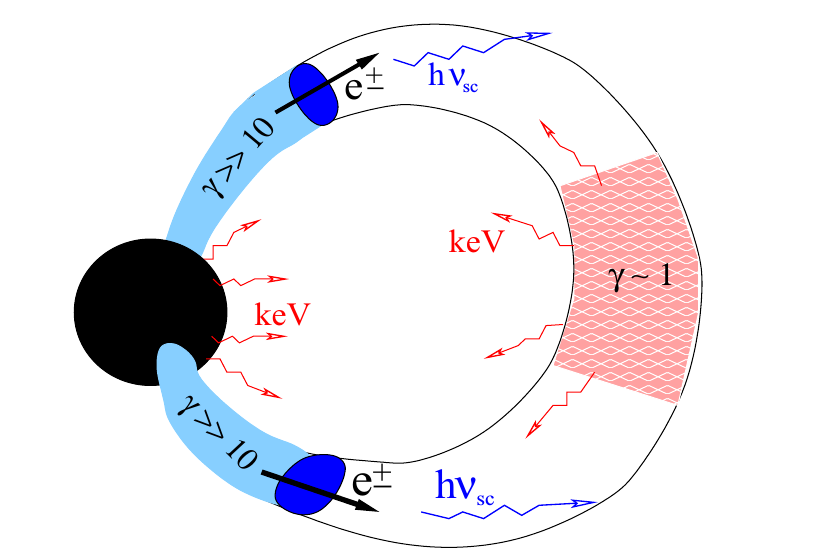
\includegraphics[width=0.7\textwidth]{magnetar.png}
    \caption{Magnetar Magnetosphere}
    \label{fig:magnetar}
\end{figure}

The twist on the magnetic field lines requires current on the field lines, as we discussed. Seed particles will be extracted from the star, and they will be accelerated to high Lorentz factors. Assuming the star provides $\sim$keV target thermal photons, they will be resonantly scattered if the Lorentz factor is such that
\begin{equation}
    \label{eq:86}
    \gamma E_t = \hbar \omega_B = bm_ec^2
\end{equation}
For normal magnetar magnetic field we need Lorentz factors of $10^3$ to $10^4$. The voltage we need will simply be
\begin{equation}
    \label{eq:85}
    e\Phi_e = \gamma_\mathrm{sc}m_ec^2 \sim 10^9\text{-}10^{10}\,\mathrm{V}
\end{equation}
The luminosity will simply be the current in the twist times the voltage drop, $L = I\Phi_e$. The way to estimate the current for a field line bundle extending to radius $R_1$ is the follows:
\begin{equation}
    \label{eq:87}
    I_1 \approx \frac{c\psi F_1}{8\pi R_1} = \frac{c\mu \psi}{4R_1^2}
\end{equation}
where $\mu$ is the magnetic moment. The typical luminosity is
\begin{equation}
    \label{eq:88}
    L\approx 10^{36}\psi \left( \frac{\mu}{10^{33}\,\mathrm{G\,cm^2}} \right)^{1/3} \left( \frac{\Phi_e}{4\times 10^9,\mathrm{V}} \right) \left( \frac{B_1}{10^{12}\, \mathrm{G}} \right)^{2/3}\,\mathrm{erg/s}
\end{equation}
which agrees with observed luminosity. We assume $R_1\sim 10R_{*}$. This is because on the field lines closer to the star the hard photons won't be able to escape and they go to pairs. The other reason is that the inner region tends to be erased sooner as when the field untwists, a cavity develops from the inner part.

We can find the timescale for untwisting by comparing the power and the total magnetic energy
\begin{equation}
    \label{eq:89}
    E_\mathrm{twist} = \int \frac{B_{\phi}^2}{8\pi}\,dV = \frac{\mu^2\psi^2u_1^3}{6R^3_{*}}
\end{equation}
where $u = \sin^2\theta = f/f_\mathrm{max}$ and $u_1$ is the $f$ on the most extended field line of the twist. Since the energy scales with $u^3$, the smaller polar angle the twist, the smaller the energy you can store. Now the dissipation timescale will simply be
\begin{equation}
    \label{eq:90}
    t_\mathrm{decay} \sim \frac{E_\mathrm{twist}}{L} = \frac{\mu^2\psi^2u_1^3}{6R^3_{*}}\frac{4R_1^2}{c\mu \psi} = \frac{\mu u_1}{cR_{*}\Phi_e} \sim 10\,\mathrm{yr}\Phi_{10}^{-1}B_{p,15}\psi u_1
\end{equation}
Note that $R_1$ is simply the $R_\mathrm{max}$ of $u_1$, in other words $u_1 = R_{*}/R_1$.

If we look at the more detailed equation of evolution of the twist, and assume there is some pumping of the twist due to shearing of the surface $\omega(f)$,
\begin{equation}
    \label{eq:91}
    \left.\partial_t\psi\right|_f = 2\pi\frac{\partial\Phi_e}{\partial f} + \omega(f)
\end{equation}
then the condition for successful pumping of the twist will be such that
\begin{equation}
    \label{eq:92}
    \omega > \frac{\psi}{t_\mathrm{decay}} \sim \frac{c R\Phi_e}{\mu u_1}
\end{equation}
The critical rate will be something like $1\,\mathrm{rad/yr}$. It is easier to twist the field if the twist is large ($u_1$ is large).

We don't know exactly what is $\Phi_e(f)$, but we have some arguments to see its behavior.


\end{document}


%%% Local Variables:
%%% mode: latex
%%% TeX-master: t
%%% End:
